\documentclass[11pt,letterpaper]{article}
\usepackage[T1]{fontenc}
\usepackage{lmodern,microtype,amsmath,amssymb,graphicx,booktabs,tabularx,array,enumitem,xcolor,fancyhdr,titlesec,tcolorbox,caption}
\tcbuselibrary{breakable}
\usepackage[margin=.8in,headheight=15pt,headsep=18pt,footskip=25pt]{geometry}
\usepackage[colorlinks=true,urlcolor=teal,linkcolor=olive]{hyperref}
\definecolor{olive}{HTML}{536240}\definecolor{ink}{HTML}{293329}\definecolor{teal}{HTML}{17677A}\definecolor{gold}{HTML}{A55C21}\definecolor{soft}{HTML}{EEF3E8}\definecolor{warm}{HTML}{FBEFDF}
\color{ink}\setlength{\parindent}{0pt}\setlength{\parskip}{7pt}
\setlist{leftmargin=1.4em,itemsep=3pt,topsep=3pt}
\renewcommand{\thesection}{8.\arabic{section}}
\titleformat{\section}{\Large\bfseries\color{olive}}{\thesection}{.6em}{}
\titleformat{\subsection}{\large\bfseries\color{teal}}{}{0pt}{}
\titlespacing*{\section}{0pt}{4pt}{12pt}\titlespacing*{\subsection}{0pt}{11pt}{4pt}
\pagestyle{fancy}\fancyhf{}\fancyhead[L]{\small\sffamily MATH\& 107 / WEEK 8 / PART I}\fancyhead[R]{\small\sffamily Feasible Choices and Convex Geometry}\fancyfoot[L]{\small\sffamily Math in Society / Dr Lee}\fancyfoot[R]{\small\sffamily\thepage}\renewcommand{\headrulewidth}{.3pt}
\tcbset{boxrule=.5pt,arc=2mm,left=10pt,right=10pt,top=7pt,bottom=7pt,before skip=9pt,after skip=9pt,colframe=olive!35,colback=soft,fonttitle=\bfseries,coltitle=teal,colbacktitle=soft}
\newcolumntype{Y}{>{\raggedright\arraybackslash}X}
\captionsetup{font=small,labelformat=empty,textfont={color=teal},skip=7pt}
\hypersetup{pdftitle={Week 8, Part I: Feasible Choices and Convex Geometry},pdfauthor={MATH and 107 / Dr Lee}}
\usepackage{needspace}
\pdfinfoomitdate=1
\pdftrailerid{}
\pdfsuppressptexinfo=15
\setlength{\emergencystretch}{2em}

\begin{document}
{\small\sffamily\color{olive}WEEK 8 / PART I / CONVEX GEOMETRY\par}
\vspace{10pt}
{\fontsize{31}{35}\selectfont\bfseries\color{olive}What is possible?\par}
\vspace{8pt}
{\large Turn resource limits into a picture of allowable plans. Learn what a point means, what a boundary means, and why every condition must hold.\par}
\begin{center}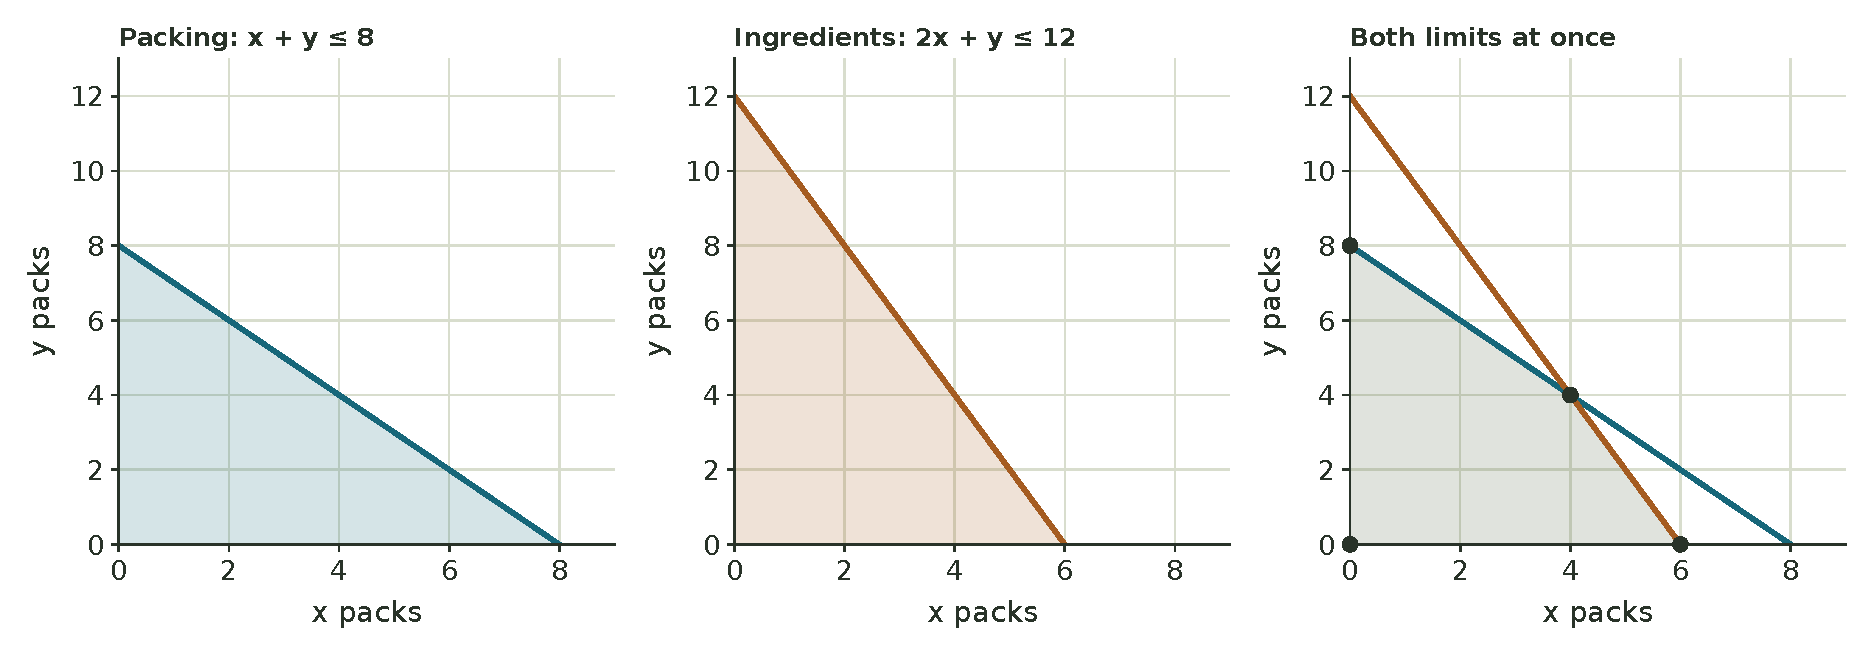
\includegraphics[width=\linewidth]{../assets/week8/constraints-overlap.pdf}\end{center}
\begin{tcolorbox}[title={The setting for the week}]
A school club makes two kinds of snack packs. It has eight packing slots and twelve ingredient portions. Type A uses twice as many portions as type B. Which complete production plans can it actually carry out?
\end{tcolorbox}
Week 7 compared costs, revenue, and profit. Here we add limits. Use multiplication, fractions, coordinate pairs, and simple equations to describe what is allowed before choosing what is best. No previous study of linear programming is assumed.

By the end of Part I, you can define variables and units, test a plan, draw a boundary and its permitted side, locate every feasible corner, and explain why the continuous region is convex. Part II uses that region to compare objectives and identify the limits of the method.

\medskip
\href{https://bobovski66.github.io/MathInSociety/readings/week8_reading.html}{Complete online reading}\quad\textperiodcentered\quad\href{https://bobovski66.github.io/MathInSociety/demos/convex_geometry.html}{Feasible-region explorer}\quad\textperiodcentered\quad\href{https://bobovski66.github.io/MathInSociety/labs/week8_lab.html}{Guided laboratory}

\clearpage


\Needspace{6\baselineskip}\section{One point records one complete plan}

Let \(x\) be the number of type-A snack packs and \(y\) the number of type-B packs. These are \emph{decision variables}: quantities the club chooses. The plan \((4,4)\) means four of A and four of B. The first coordinate is always \(x\); the second is \(y\).


On the graph, move horizontally to the x-value, then vertically to the y-value. The point is a whole production plan, not a moment in time. The line between two plans will later represent mixtures or averages of those plans.



\par\medskip\noindent\begin{minipage}{\linewidth}
\centering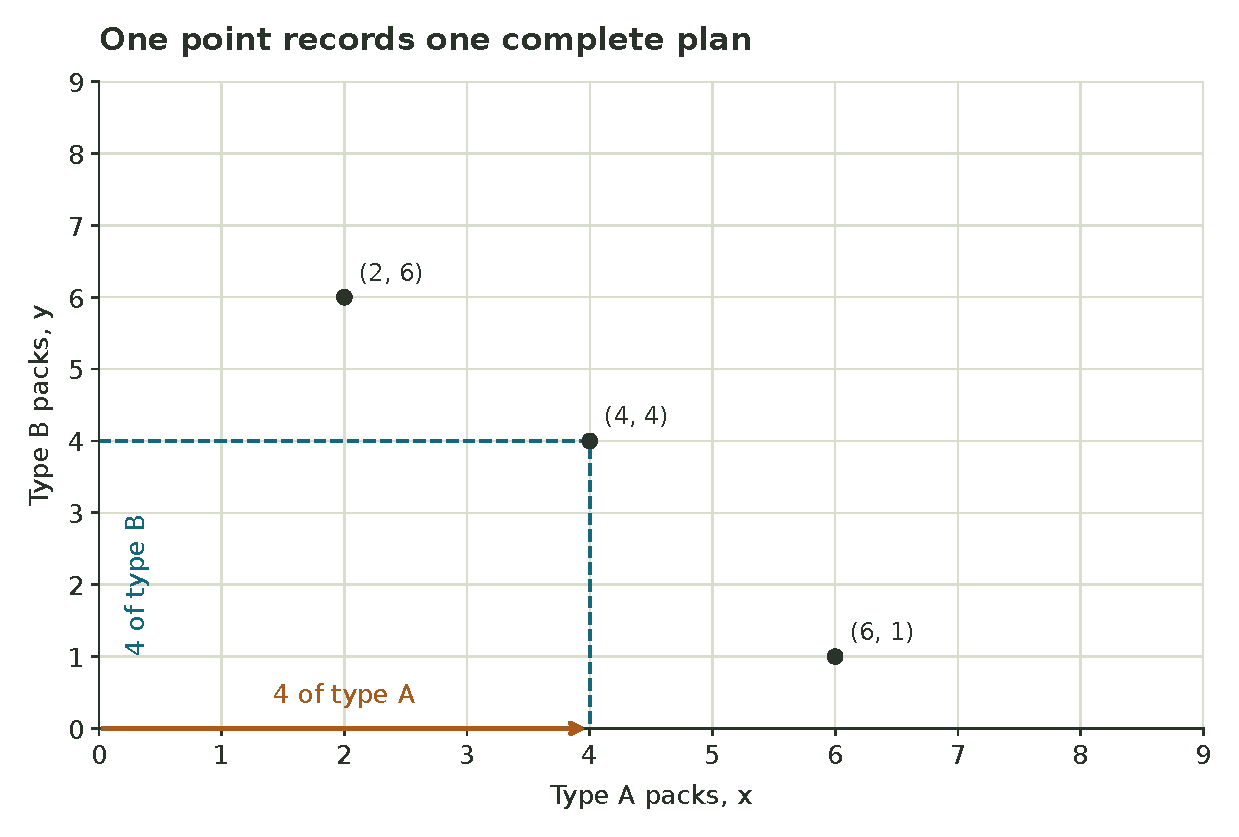
\includegraphics[width=\linewidth,height=3.2in,keepaspectratio]{../assets/week8/plan-coordinates.pdf}
\captionof*{figure}{Read (2,6) as ``2 type-A packs and 6 type-B packs.'' This is a graph of choices. Neither axis measures time, and a higher point is not automatically a better plan.}
\end{minipage}\par\medskip

\par\medskip{\small\renewcommand{\arraystretch}{1.35}\begin{tabularx}{\linewidth}{@{}YYYY@{}}\toprule
Per pack or resource & Type A, x & Type B, y & Available\\
\midrule
Packing slots & 1 & 1 & 8 slots\\
Ingredient portions & 2 & 1 & 12 portions\\
Fundraiser contribution &  \$3 &  \$2 & This is what we want to increase\\
\bottomrule\end{tabularx}}\par\medskip


The resource counts and contribution amounts are invented for this example. A contribution is the amount left after the per-pack costs in Week 7. If there is also a fixed event expense, subtracting the same fixed amount from every plan changes the reported profit but does not change which plan has the largest contribution.


\begin{tcolorbox}[title={The drawing and the actual products},breakable,colback=warm,colbacktitle=warm,coltitle=gold,colframe=gold!35]

For geometry, we first allow nonnegative real values of \(x\) and \(y\), including fractions. Real snack packs must be whole. Later we will check that requirement separately. Our main example's best plan happens to be whole-numbered, so it is usable in both models.


\end{tcolorbox}


\begin{tcolorbox}[title={Pause and try 1},breakable]
What does (5,2) mean? What would (2,5) mean, and why is it a different decision?
\end{tcolorbox}


\Needspace{6\baselineskip}\section{Each constraint compares a total with a limit}

Each pack uses one packing slot, so making \(x\) of A and \(y\) of B uses \(x+y\) slots. With at most eight available, the club needs \(x+y\leq8\). The symbol \(\leq\) means ``less than or equal to'': using all eight is allowed, but using nine is not.


A type-A pack uses two ingredient portions and a type-B pack uses one. Their total use is \(2x+y\), giving \(2x+y\leq12\). The coefficient 2 means \emph{2 portions per pack}. Multiplying by \(x\) packs gives portions; both sides of this comparison have the same units.

\[x+y\leq8,\qquad 2x+y\leq12,\qquad x\geq0,\quad y\geq0.\]
The last two constraints forbid negative production. A plan is \emph{feasible} if it satisfies \emph{every} constraint. Passing one test is not enough.


\begin{tcolorbox}[title={Example \textperiodcentered{} Test (5,3) and (3,3)},breakable]

At (5,3), packing uses \(5+3=8\) slots, which is allowed. Ingredients use \(2(5)+3=13\) portions, which exceeds 12. The plan is infeasible despite passing the packing test.


At (3,3), packing uses 6 and ingredients use 9; both coordinates are nonnegative. This plan is feasible. It leaves 2 packing slots and 3 ingredient portions unused. These unused amounts are called \emph{slack} for the upper limits.


\end{tcolorbox}


\par\medskip{\small\renewcommand{\arraystretch}{1.35}\begin{tabularx}{\linewidth}{@{}YYY@{}}\toprule
Words & Mathematical form & Meaning\\
\midrule
At most 8 & total $\le$ 8 & 8 is allowed; larger totals are not\\
At least 8 & total $\ge$ 8 & 8 is allowed; smaller totals are not\\
Exactly 8 & total = 8 & Only 8 is allowed\\
Less than 8 & total \textless{} 8 & 8 itself is excluded\\
\bottomrule\end{tabularx}}\par\medskip


A constraint is \emph{binding}, or active, at a plan when it holds with equality. At (4,4), both resource limits bind: \(4+4=8\) and \(2(4)+4=12\). A binding constraint has no slack at that plan.



\begin{tcolorbox}[title={Pause and try 2},breakable]
Does (6,1) satisfy the club's full system? Show both resource calculations.
\end{tcolorbox}

\clearpage

\Needspace{6\baselineskip}\section{The boundary is a line; the inequality permits a whole side}

First consider a separate practice inequality, \(x+2y\leq8\). Its \emph{boundary line} is \(x+2y=8\). An equality identifies the plans that use exactly the limit; the inequality also includes plans using less.


\begin{tcolorbox}[title={Example \textperiodcentered{} Find two intercepts, then test one point},breakable]

\begin{enumerate}
\item Set \(y=0\): then \(x=8\), giving the x-intercept (8,0).
\item Set \(x=0\): then \(2y=8\), so \(y=4\), giving the y-intercept (0,4).
\item Draw the line through those points.
\item Test a point off the line. At (0,0), \(0+2(0)=0\leq8\), so the side containing the origin is permitted.

\end{enumerate}

\end{tcolorbox}


\par\medskip\noindent\begin{minipage}{\linewidth}
\centering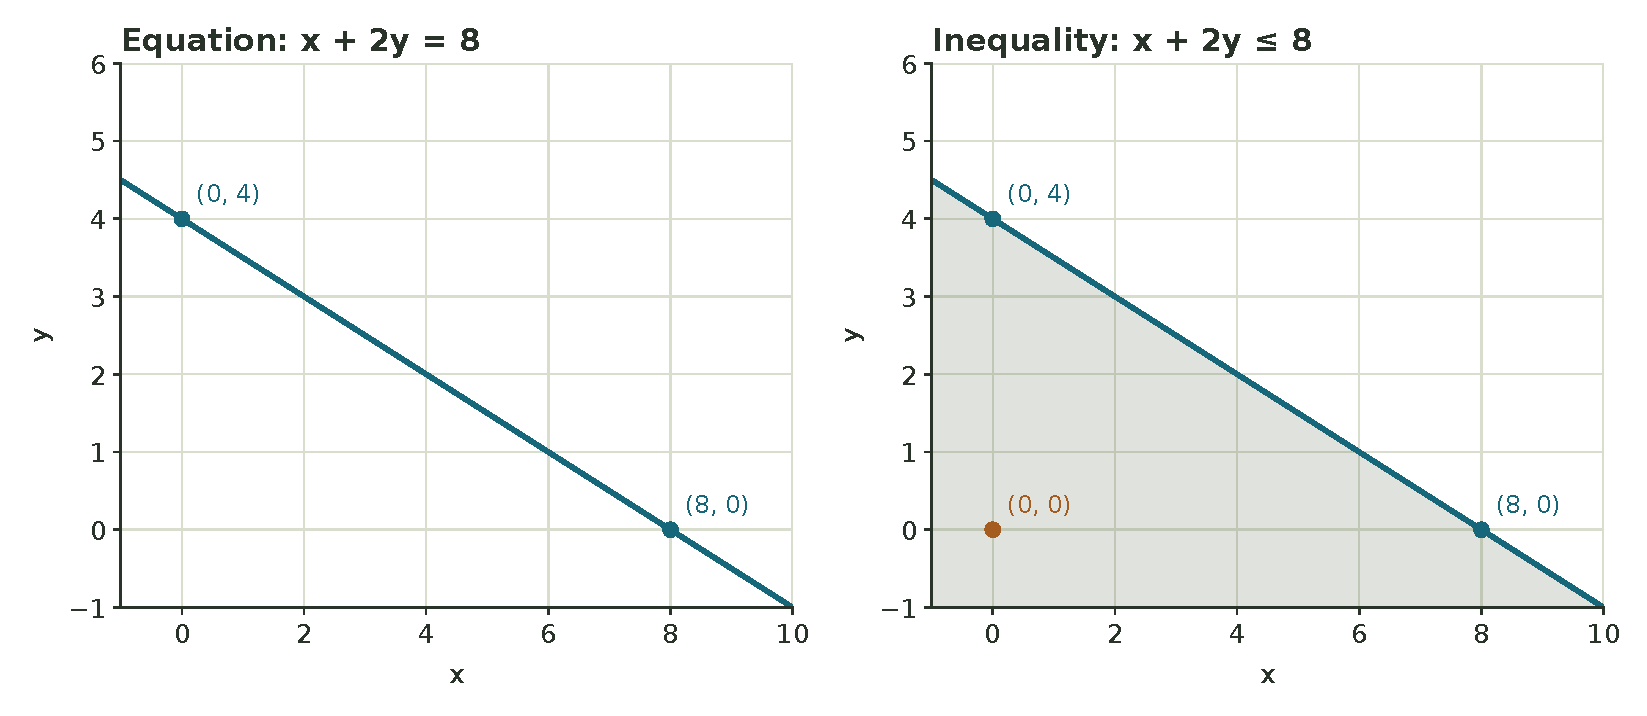
\includegraphics[width=\linewidth,height=3.2in,keepaspectratio]{../assets/week8/half-plane.pdf}
\captionof*{figure}{The equation describes a line. The inequality describes a half-plane: that line together with all points on one side. The panels show only a window of the plane; a half-plane continues beyond the picture.}
\end{minipage}\par\medskip


For \(\leq\) or \(\geq\), draw the boundary as a solid line because equality is allowed. For a strict inequality, such as \(<\), use a dashed boundary to show exclusion. Our optimization examples use included boundaries. If the origin lies on the boundary, choose a different test point that does not.


In the club model, \(x\geq0\) and \(y\geq0\) restrict us to the \emph{first quadrant including its axes}. This restriction does not make a single half-plane a bounded region on its own; we must inspect all the conditions together.



\begin{tcolorbox}[title={Pause and try 3},breakable]
For x + 2y $\le$ 8, is (2,3) on the boundary, strictly on the permitted side, or outside? What about (4,3)?
\end{tcolorbox}

\clearpage

\Needspace{6\baselineskip}\section{The feasible region is the overlap}

Return to the club's limits, \(x+y\leq8\) and \(2x+y\leq12\), with nonnegative coordinates. Each limit permits its own side of a boundary. The \emph{feasible region} is their \emph{intersection}: the points common to all the permitted sets.



\par\medskip\noindent\begin{minipage}{\linewidth}
\centering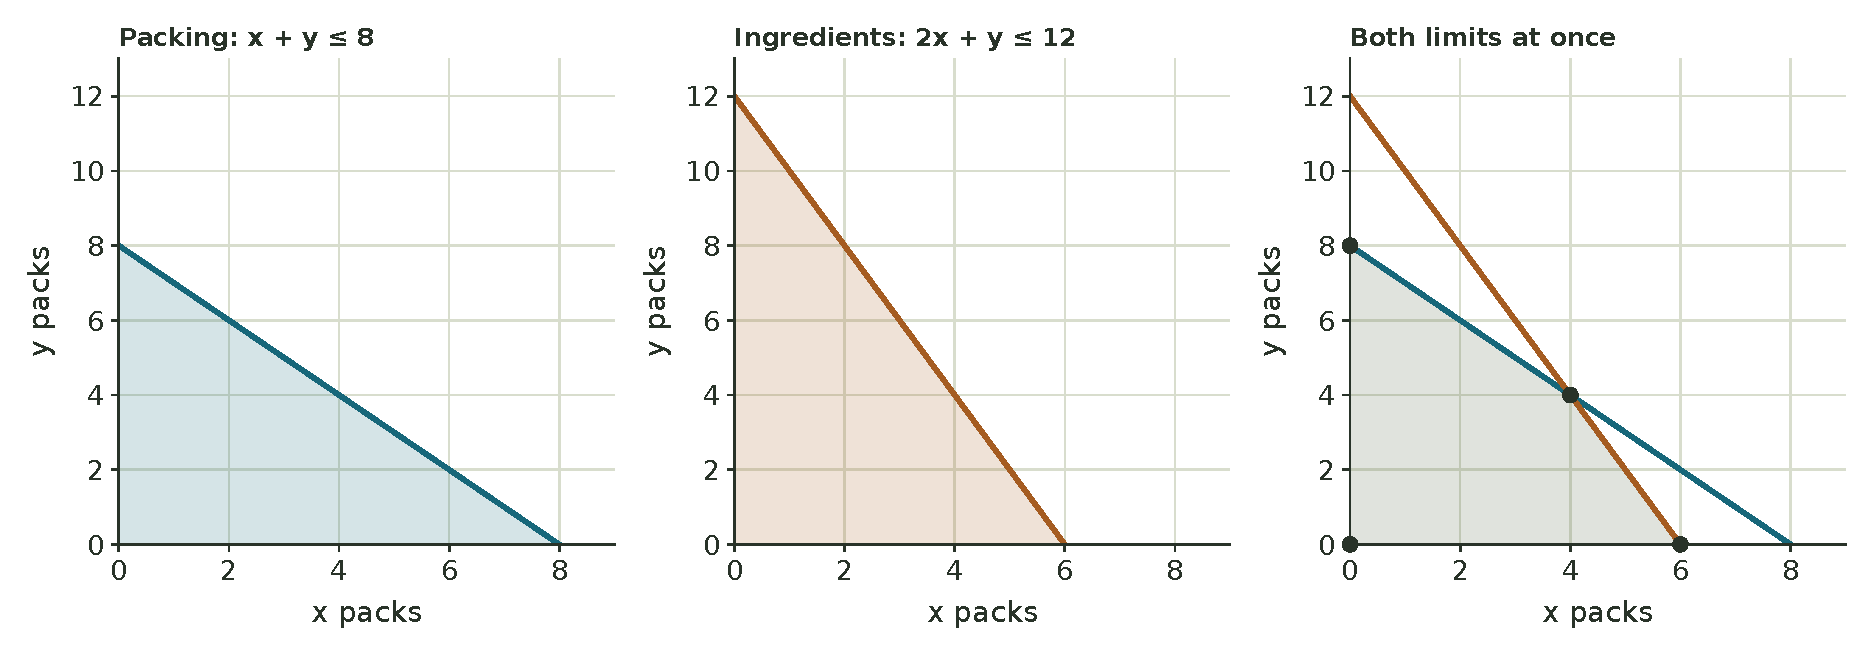
\includegraphics[width=\linewidth,height=3.2in,keepaspectratio]{../assets/week8/constraints-overlap.pdf}
\captionof*{figure}{The first two panels show one resource limit at a time, with nonnegative coordinates. Keep a plan only if it is permitted in both panels. The final shaded polygon is the feasible region.}
\end{minipage}\par\medskip


A \emph{vertex} (plural: vertices) is a corner of this region. Corners come from intersecting boundaries, including the axes. A boundary intersection is only a \emph{candidate} vertex until we verify all constraints.


\begin{tcolorbox}[title={Example \textperiodcentered{} Find the non-axis corner},breakable]

Solve the two resource boundaries simultaneously:


\[x+y=8,\qquad 2x+y=12.\]


Subtract the first equation from the second: \((2x+y)-(x+y)=12-8\), so \(x=4\). Substitute into \(x+y=8\) to get \(y=4\). Thus the boundaries meet at (4,4). Both coordinates are nonnegative, so this intersection is feasible.


On the x-axis, \(y=0\). The limits require both \(x\leq8\) and \(x\leq6\), so the tighter upper limit is 6. The x-axis corner is (6,0). On the y-axis, the tighter limit is 8, giving (0,8). The origin is the fourth corner.


\end{tcolorbox}


\par\medskip\noindent\begin{minipage}{\linewidth}
\centering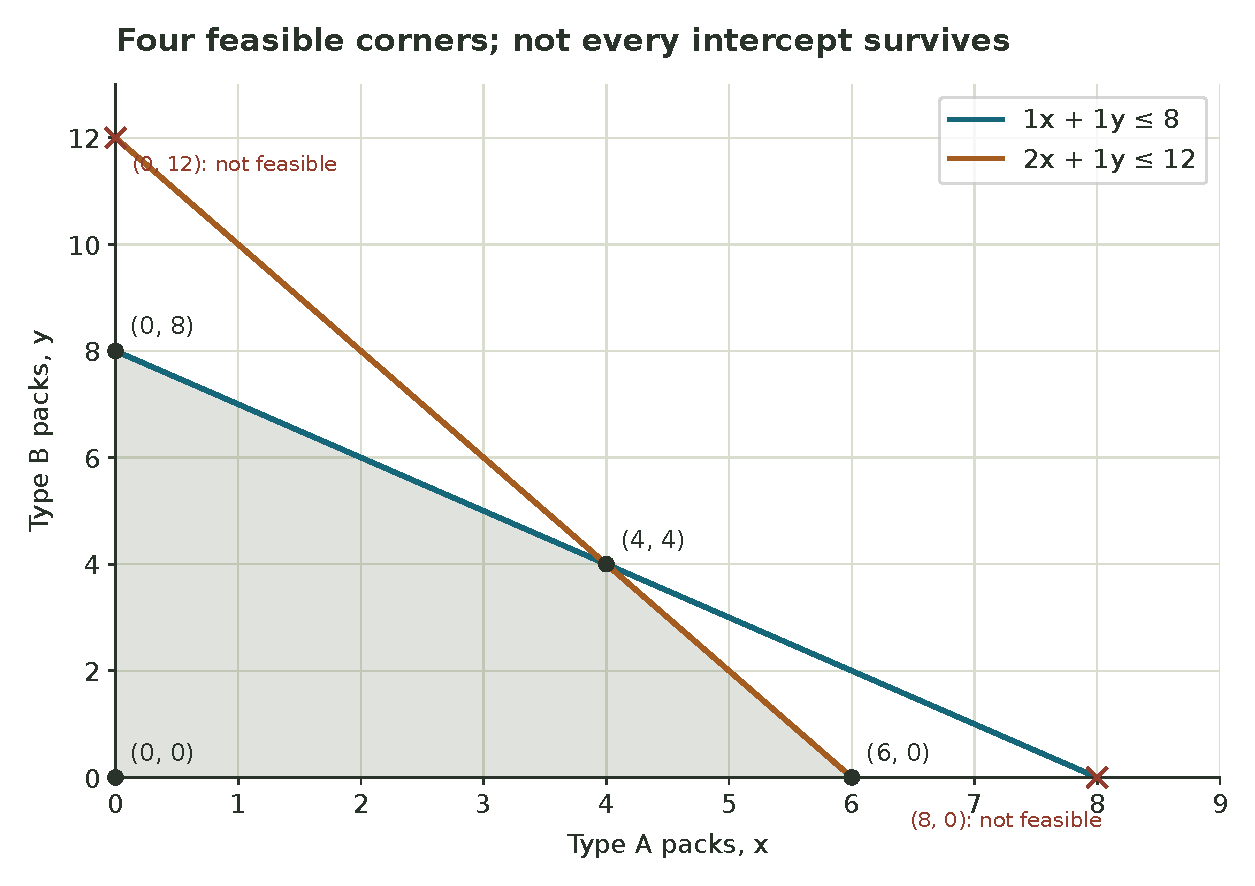
\includegraphics[width=\linewidth,height=3.8in,keepaspectratio]{../assets/week8/feasible-vertices.pdf}
\captionof*{figure}{Two different ideas: (8,0) is an intercept of the packing boundary, but it is not a feasible corner because it needs 16 ingredient portions. Likewise, (0,12) violates the packing limit.}
\end{minipage}\par\medskip

\par\medskip{\small\renewcommand{\arraystretch}{1.35}\begin{tabularx}{\linewidth}{@{}YYYY@{}}\toprule
Corner & Packing use x+y $\le$ 8 & Ingredient use 2x+y $\le$ 12 & Binding resource limits\\
\midrule
(0,0) & 0 & 0 & Neither\\
(6,0) & 6 & 12 & Ingredients\\
(4,4) & 8 & 12 & Both\\
(0,8) & 8 & 8 & Packing\\
\bottomrule\end{tabularx}}\par\medskip


The axes are also boundaries: at (6,0), for example, the nonnegativity condition \(y\geq0\) binds along with the ingredient limit. A corner does not always use up both resources.



\begin{tcolorbox}[title={Pause and try 4},breakable]
For x+y$\le$7 and 2x+y$\le$10 with x,y$\ge$0, find the intersection of the two non-axis boundaries. Is (7,0) a feasible corner?
\end{tcolorbox}


\Needspace{6\baselineskip}\section{Convexity means that the whole segment stays inside}

A set is \emph{convex} if the straight segment between \emph{any two} points in the set remains entirely in the set. A filled triangle, filled rectangle, and filled disk are convex. A ring is not: a segment across the hole leaves the set. The circumference of a circle alone is also not convex; the disk includes the interior.



\par\medskip\noindent\begin{minipage}{\linewidth}
\centering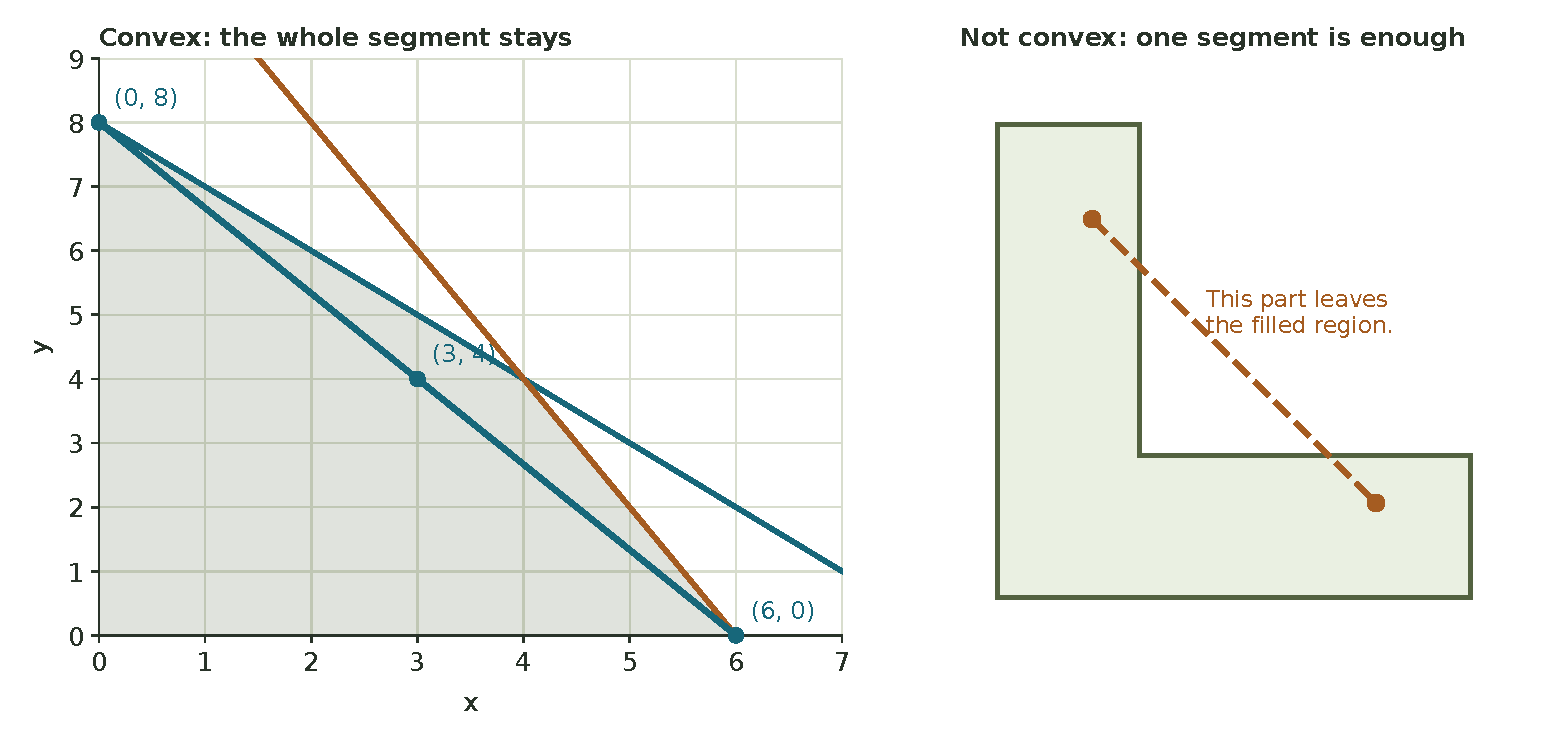
\includegraphics[width=\linewidth,height=3.2in,keepaspectratio]{../assets/week8/convex-segments.pdf}
\captionof*{figure}{To establish nonconvexity, one counterexample segment is enough. Convexity requires every such segment to remain inside, not just one convenient segment.}
\end{minipage}\par\medskip


\begin{tcolorbox}[title={Example \textperiodcentered{} Average two feasible plans},breakable]

The halfway plan between (6,0) and (0,8) is \(((6+0)/2,(0+8)/2)=(3,4)\). It uses \(3+4=7\) packing slots and \(2(3)+4=10\) ingredient portions, both within the limits.


Why does averaging work for any two feasible real-valued plans? Each resource total at the average plan is the average of the two resource totals. If each total is at most a limit, their average is too. The same reasoning works for any mixture with nonnegative weights adding to 1.


\end{tcolorbox}

Every half-plane is convex, and intersections of convex sets are convex. This explains the shape of our feasible region. A \emph{union} is different: two separated filled rectangles are individually convex, but taking all points in either rectangle produces a set with a gap.


Whole-number plans are a separate issue: the halfway plan between (1,0) and (0,1) is (0.5,0.5), which is not a whole-number production plan. Convexity applies to the continuous region we drew, not to the isolated integer points within it.



\begin{tcolorbox}[title={Pause and try 5},breakable]
Why is a filled rectangle convex while two separated filled rectangles, taken together, are not?
\end{tcolorbox}

\clearpage
\section*{Part I Review}
Use nonnegative real coordinates unless the question explicitly asks for whole numbers. Show a substitution, boundary calculation, or segment argument.
\begin{enumerate}
\item Define variables for a workshop making chairs and tables. What does the plan $(5,2)$ mean? Explain why $(2,5)$ is different.
\item A type-A item uses 3 labor-hours and a type-B item 2. Write a 60-hour upper limit with units. Test $(10,10)$ and $(15,8)$ and report slack or the shortfall.
\item For $x+2y\leq8$, find both boundary intercepts. Identify the permitted side by testing a point off the boundary. Classify $(2,3)$ and $(4,3)$.
\item Find every feasible corner for $x+y\leq7$, $2x+y\leq10$, $x,y\geq0$. Show the intersection calculation. Why is $(7,0)$ not a corner of the feasible region?
\item Find the corners for $3x+2y\leq120$, $x+2y\leq60$, $x,y\geq0$. Test $(20,20)$ and $(25,20)$ against both resource limits.
\item For the workshop constraints $2x+4y\leq40$, $x+y\leq14$, find the four corners. Check proposed plans $(8,5)$ and $(10,5)$.
\item Which sets are convex: a filled disk, a circle's circumference alone, a filled rectangle, a ring, a line segment? Explain a counterexample segment for each nonconvex set.
\item Why is an intersection of convex sets convex? Give a counterexample showing that a union need not be convex.
\item For the club's region, average $(6,0)$ and $(0,8)$. Check the resulting plan against $x+y\leq8$ and $2x+y\leq12$. Why need a midpoint of two whole-number plans not be a whole-number plan?
\item Keep the club's packing limit at 8 and raise the ingredient allowance from 12 to 16. Do old feasible plans remain feasible? Give one newly feasible plan.
\item If $x+y\leq8$ is already imposed, does adding $x+y\leq10$ remove any choices? What does it mean for a constraint to be redundant?
\item Describe the feasible sets for (a) $x+y\leq4$ and $x+y\geq6$; (b) $x+y\leq0$ with $x,y\geq0$. Why should we not assume every system creates a filled four-sided polygon?
\end{enumerate}

\clearpage
{\setlength{\parskip}{4pt}\setlist{itemsep=4pt,topsep=3pt}\titlespacing*{\paragraph}{0pt}{5pt}{.75em}
\section*{Solutions and Reasoning}

\paragraph{Short check 1.}
The first means 5 type-A packs and 2 type-B packs; the second means 2 of A and 5 of B. The products have different ingredient use and contributions, so exchanging the coordinates changes the plan.


\paragraph{Short check 2.}
Packing uses 6+1 = 7 $\le$ 8, but ingredients use 2(6)+1 = 13 \textgreater{} 12. It is not feasible. A single violated constraint rules out a plan.


\paragraph{Short check 3.}
At (2,3), 2+2(3)=8, so it is on the included boundary. At (4,3), the total is 10, so it is outside. An included boundary point is feasible for that inequality.


\paragraph{Short check 4.}
Subtracting gives x=3, then y=4, so the intersection is (3,4). The intercept (7,0) fails 2x+y$\le$10 because it uses 14. The feasible x-axis corner is (5,0).


\paragraph{Short check 5.}
A segment between any two points in one filled rectangle stays in that rectangle. With two separated rectangles, choose one point in each: the connecting segment crosses a gap outside their union.



\subsection*{Part I Review: solutions}
\begin{enumerate}
\item Let $x$ count chairs per week and $y$ tables per week. $(5,2)$ means five chairs and two tables. Switching the coordinates switches the products, which may change resource use and value.
\item $3x+2y\leq60$ hours, where the coefficients are hours per item. $(10,10)$ uses $30+20=50$ hours, leaving 10. $(15,8)$ uses $45+16=61$ hours and exceeds the allowance by 1.
\item Intercepts are $(8,0)$ and $(0,4)$. The origin gives $0\leq8$, so its side is permitted. $(2,3)$ is on the included boundary; $(4,3)$ is outside because its total is 10.
\item Subtract $x+y=7$ from $2x+y=10$: $x=3$, then $y=4$. Corners are $(0,0),(5,0),(3,4),(0,7)$. $(7,0)$ uses 14 under the second limit, exceeding 10.
\item Subtract the resource equations to get $2x=60$, so $x=30,y=15$. Corners are $(0,0)$, $(40,0)$, $(30,15)$, and $(0,30)$. At $(20,20)$, use is 100 and 60: feasible. At $(25,20)$, use is 115 and 65: the second limit fails.
\item Divide the first boundary by 2 and subtract $x+y=14$ from $x+2y=20$, obtaining $y=6,x=8$. Corners are $(0,0),(14,0),(8,6),(0,10)$. $(8,5)$ uses 36 wood units and 13 slots: feasible. $(10,5)$ uses 40 wood units but 15 slots: infeasible.
\newpage
\item The filled disk, filled rectangle, and line segment are convex. Opposite points of a circle's circumference have a segment through the missing interior. Opposite sides of a ring have a segment through the hole. These counterexamples establish nonconvexity.
\item If two points lie in every set, their joining segment lies in every convex set and thus in the intersection. For a union, take two separated filled rectangles and join a point of one to a point of the other: the segment crosses a gap.
\item The midpoint is $(3,4)$, using 7 slots and 10 ingredient portions. It is feasible. But the midpoint of whole-number points $(1,0)$ and $(0,1)$ is $(0.5,0.5)$, which is not a whole-number plan.
\item Every old feasible plan remains feasible because the ingredient upper limit is relaxed. $(8,0)$ is newly feasible: it uses 8 slots and 16 portions.
\item No choices are removed: a total at most 8 is automatically at most 10. A redundant constraint adds no restriction beyond those already imposed.
\item (a) The set is empty: one total cannot be at most 4 and at least 6. (b) Only $(0,0)$ is feasible. Other systems can produce triangles, larger polygons, line segments, or unbounded sets. The shape must be established from the actual conditions.
\end{enumerate}
\subsection*{Continue with Part II}
Now add an objective to the feasible region. The online optimizer and Part II explain which conditions justify a corner comparison, what ties mean, and why the best continuous plan may not be a usable whole-number plan.
}
\end{document}
